\documentclass{article}
\usepackage{iclr2027_conference,times}
\usepackage[T1]{fontenc}
\usepackage[utf8]{inputenc}
\usepackage{amsmath,amssymb,graphicx,booktabs,longtable}
\usepackage{hyperref}
\usepackage{url}
\makeatletter
\let\inputrows\@@input
\makeatother
% Generated by export_tex.py from actual saved outputs.
\newcommand{\WD}{1.58}
\newcommand{\WDLo}{0.99}
\newcommand{\WDHi}{2.02}
\newcommand{\WRelative}{4.85}
\newcommand{\WRelativeLo}{2.70}
\newcommand{\WRelativeHi}{7.51}
\newcommand{\WTrain}{0.60}
\newcommand{\WTrainLo}{0.60}
\newcommand{\WTrainHi}{0.60}
\newcommand{\WGen}{0.124}
\newcommand{\WGenLo}{0.080}
\newcommand{\WGenHi}{0.222}
\newcommand{\WPadj}{0.0234}
\newcommand{\WNinetyFive}{0.60}
\newcommand{\WNinetyFiveLo}{0.31}
\newcommand{\WNinetyFiveHi}{0.85}
\newcommand{\WNinety}{0.22}
\newcommand{\WNinetyLo}{0.07}
\newcommand{\WNinetyHi}{0.37}
\newcommand{\WideD}{-0.172}
\newcommand{\WideDLo}{-0.269}
\newcommand{\WideDHi}{-0.083}
\newcommand{\KSmall}{-0.057}
\newcommand{\KSmallLo}{-0.170}
\newcommand{\KSmallHi}{0.000}
\newcommand{\KSmallP}{1.00}
\newcommand{\ClockSmallRestrictedRatio}{0.943}
\newcommand{\ClockSmallRestrictedRatioLo}{0.830}
\newcommand{\ClockSmallRestrictedRatioHi}{1.000}
\newcommand{\KLarge}{-0.003}
\newcommand{\KLargeLo}{-0.009}
\newcommand{\KLargeHi}{0.004}
\newcommand{\KLargeP}{1.00}
\newcommand{\ClockLargeRestrictedRatio}{0.986}
\newcommand{\ClockLargeRestrictedRatioLo}{0.952}
\newcommand{\ClockLargeRestrictedRatioHi}{1.023}
\newcommand{\ClockLargeRatio}{1.005}
\newcommand{\ClockLargeRatioLo}{0.964}
\newcommand{\ClockLargeRatioHi}{1.048}
\newcommand{\NormMeanD}{1.54}
\newcommand{\NormMeanDLo}{1.01}
\newcommand{\NormMeanDHi}{2.08}
\newcommand{\NormMatchedD}{0.92}
\newcommand{\NormMatchedDLo}{0.61}
\newcommand{\NormMatchedDHi}{1.25}
\newcommand{\CPUHours}{3.43}
\newcommand{\RunSecondsMin}{32.1}
\newcommand{\RunSecondsMax}{830.0}
\newcommand{\ElapsedMinutes}{57.5}
\newcommand{\HalfLargeFinalMean}{95.7}
\newcommand{\HalfLargeFinalMin}{88.2}
\newcommand{\HalfLargeFinalEvents}{1}
\newcommand{\HalfLargeRegressions}{7}
\newcommand{\MainTinyTrain}{100.0}
\newcommand{\MainTinyTrainLo}{100.0}
\newcommand{\MainTinyTrainHi}{100.0}
\newcommand{\MainTinyEval}{43.3}
\newcommand{\MainTinyEvalLo}{37.9}
\newcommand{\MainTinyEvalHi}{49.0}
\newcommand{\MainTinyTrainEvents}{8}
\newcommand{\MainTinyEvalEvents}{0}
\newcommand{\MainTinyIncLo}{0.0}
\newcommand{\MainTinyIncHi}{32.4}
\newcommand{\MainNarrowTrain}{100.0}
\newcommand{\MainNarrowTrainLo}{100.0}
\newcommand{\MainNarrowTrainHi}{100.0}
\newcommand{\MainNarrowEval}{73.5}
\newcommand{\MainNarrowEvalLo}{69.1}
\newcommand{\MainNarrowEvalHi}{77.9}
\newcommand{\MainNarrowTrainEvents}{8}
\newcommand{\MainNarrowEvalEvents}{0}
\newcommand{\MainNarrowIncLo}{0.0}
\newcommand{\MainNarrowIncHi}{32.4}
\newcommand{\MainSmallTrain}{100.0}
\newcommand{\MainSmallTrainLo}{100.0}
\newcommand{\MainSmallTrainHi}{100.0}
\newcommand{\MainSmallEval}{98.6}
\newcommand{\MainSmallEvalLo}{98.0}
\newcommand{\MainSmallEvalHi}{99.3}
\newcommand{\MainSmallTrainEvents}{8}
\newcommand{\MainSmallEvalEvents}{2}
\newcommand{\MainSmallIncLo}{7.1}
\newcommand{\MainSmallIncHi}{59.1}
\newcommand{\MainLargeTrain}{100.0}
\newcommand{\MainLargeTrainLo}{100.0}
\newcommand{\MainLargeTrainHi}{100.0}
\newcommand{\MainLargeEval}{100.0}
\newcommand{\MainLargeEvalLo}{100.0}
\newcommand{\MainLargeEvalHi}{100.0}
\newcommand{\MainLargeTrainEvents}{8}
\newcommand{\MainLargeEvalEvents}{8}
\newcommand{\MainLargeIncLo}{67.6}
\newcommand{\MainLargeIncHi}{100.0}
\newcommand{\CapacityTrainTrain}{100.0}
\newcommand{\CapacityTrainTrainLo}{100.0}
\newcommand{\CapacityTrainTrainHi}{100.0}
\newcommand{\CapacityTrainEval}{100.0}
\newcommand{\CapacityTrainEvalLo}{100.0}
\newcommand{\CapacityTrainEvalHi}{100.0}
\newcommand{\CapacityTrainTrainEvents}{8}
\newcommand{\CapacityTrainEvalEvents}{8}
\newcommand{\CapacityTrainIncLo}{67.6}
\newcommand{\CapacityTrainIncHi}{100.0}
\newcommand{\CapacityFrozenTrain}{100.0}
\newcommand{\CapacityFrozenTrainLo}{100.0}
\newcommand{\CapacityFrozenTrainHi}{100.0}
\newcommand{\CapacityFrozenEval}{0.1}
\newcommand{\CapacityFrozenEvalLo}{0.0}
\newcommand{\CapacityFrozenEvalHi}{0.2}
\newcommand{\CapacityFrozenTrainEvents}{8}
\newcommand{\CapacityFrozenEvalEvents}{0}
\newcommand{\CapacityFrozenIncLo}{0.0}
\newcommand{\CapacityFrozenIncHi}{32.4}
\newcommand{\FrozenLargeTrain}{100.0}
\newcommand{\FrozenLargeTrainLo}{100.0}
\newcommand{\FrozenLargeTrainHi}{100.0}
\newcommand{\FrozenLargeEval}{1.0}
\newcommand{\FrozenLargeEvalLo}{0.6}
\newcommand{\FrozenLargeEvalHi}{1.5}
\newcommand{\FrozenLargeTrainEvents}{8}
\newcommand{\FrozenLargeEvalEvents}{0}
\newcommand{\FrozenLargeIncLo}{0.0}
\newcommand{\FrozenLargeIncHi}{32.4}
\newcommand{\ShuffleLargeTrain}{100.0}
\newcommand{\ShuffleLargeTrainLo}{100.0}
\newcommand{\ShuffleLargeTrainHi}{100.0}
\newcommand{\ShuffleLargeEval}{2.6}
\newcommand{\ShuffleLargeEvalLo}{1.8}
\newcommand{\ShuffleLargeEvalHi}{3.5}
\newcommand{\ShuffleLargeTrainEvents}{8}
\newcommand{\ShuffleLargeEvalEvents}{0}
\newcommand{\ShuffleLargeIncLo}{0.0}
\newcommand{\ShuffleLargeIncHi}{32.4}

\title{When Width Shortens Grokking:\\A Censoring-Aware Study of Quadratic Networks}
\author{Anonymous authors}
% Official anonymous-review formatting; this artifact has not been submitted.
\begin{document}
\maketitle
\begin{abstract}
Does widening a model primarily accelerate memorization, leaving rule acquisition on a slower regularization clock? We formulate and test this account on exhaustive modular-arithmetic tables using 240 CPU training runs, eight paired split--initialization seeds per setting, and a protocol frozen after independent pilots. In a width-normalized quadratic network, every main-sweep width fits the training subset, but sustained 99\% held-out accuracy occurs in only 2/8 width-32 runs versus 8/8 width-128 runs within 20,000 updates. The prespecified interaction between training and held-out restricted log times has the opposite sign to the account's prediction: $\WD$ (95\% interval $[\WDLo,\WDHi]$; Holm-adjusted $p=\WPadj$). Thus widening accelerates the observable held-out endpoint more, not less, than interpolation. An exploratory 64-to-256 contrast reverses this interaction, underscoring width-range dependence. Half/double-decay interventions give inverse-clock-compatible first onsets at width 128, but seven of eight half-decay runs later end below 99\%; width-32 clock comparisons are largely censored and inconclusive. An explicit eight-unit exact classifier rules out representational impossibility as the sole explanation for narrow-model failures. Normalization, frozen-feature, label-shuffle, data-fraction and modulus controls delimit the evidence. These results concern one quadratic/AdamW recipe, not a universal scale law or a first observation of model-wise grokking.
\end{abstract}

\section{Introduction}
Grokking separates fitting a finite training table from acquiring a rule for unseen entries: training accuracy can saturate long before held-out accuracy rises \citep{power2022}. Model size could affect either transition, their difference, their ratio, or whether either transition is observed at all. These are distinct questions. A wider model can generalize sooner in absolute updates while still spending more updates after interpolation than before it. Conversely, a narrow model that fits but does not generalize within the horizon has not demonstrated a completed grokking transition.

Width-dependent grokking itself is established prior work. \citet{davies2023} report model-wise grokking in transformers on modular division; \citet{nanda2023} also examine dimension changes. Our contribution is not another claim of first observation. We instead test a narrow, falsifiable explanation in an inexpensive feature-learning model: \emph{extra width mainly accelerates fitting individual examples, while generalization remains governed by a width-insensitive regularization clock}. This combines two operational predictions, which can fail separately:
\begin{itemize}
\item \textbf{W, preferential interpolation:} widening from 32 to 128 should accelerate sustained training interpolation more than held-out acquisition. A practical target is at least a 1.25-fold relative advantage on the specified restricted endpoint.
\item \textbf{C, inverse-decay timing:} halving or doubling AdamW decay should leave generalization times approximately unchanged in the exact multiplicative-shrinkage clock, when events are observable.
\end{itemize}
Our incremental result is a replicated, restricted-time width interaction that survives lower accuracy thresholds, paired with a direct separation between clock-compatible first onset and subsequent retention. W is our operational account, not a canonical prediction attributed to the cited papers. Circuit-efficiency accounts motivate separating fast fitting from slower generalizing solutions \citep{varma2023}; norm landscapes and lazy-to-rich dynamics motivate checking scale and feature learning rather than interpreting parameter count alone \citep{liu2023,kumar2024}. These motivations do not logically imply W or C. In particular, neither a decreasing norm nor a decay-only identity proves a trained generalization mechanism.

Our experiment contradicts W for its frozen width contrast. C is compatible with first-onset observations at width 128 but unresolved at width 32, where censoring makes a near-zero contrast uninformative. Crucially, wide-model clock compatibility does not imply lasting acquisition: most half-decay runs later regress below the threshold. Width changes the observed finite-budget accuracy endpoint, and onset timing alone does not identify a serial discovery--cleanup mechanism. All conclusions are conditional on a quadratic network, synthetic pair splits and full-batch AdamW; there is no transformer or large-language-model evidence.

\section{Related Work}
\paragraph{Grokking and size.}
\citet{power2022} establish delayed generalization on small algorithmic tables and show why optimization beyond interpolation matters. \citet{davies2023} connect grokking and double descent through patterns learned at different speeds and explicitly vary transformer embedding dimension. Our paired-seed, censoring-aware analysis addresses a recipe-specific timing prediction, not the novelty of width-wise grokking. A finite-budget non-event is not evidence of eventual impossibility.

\paragraph{Progress and mechanisms.}
\citet{nanda2023} recover Fourier-based modular-addition circuits and use progress measures and causal ablations to distinguish memorization, circuit formation and cleanup. \citet{varma2023} study a slower but more norm-efficient generalizing circuit. Our exact rule-output projection is broader than a recovered sparse Fourier circuit and is only an oracle-assisted diagnostic. Neither its energy nor its residual identifies ground-truth circuit size.

\paragraph{Scale and regularization.}
\citet{liu2023} investigate norm-dependent loss landscapes and approximate inverse-decay timing in particular ranges. \citet{kumar2024} connect grokking to feature learning, including examples without explicit regularization and with increasing norms. Their gradient-descent scaling rules are not AdamW invariances. \citet{loshchilov2019} distinguish decoupled decay from L2 regularization under adaptive optimization, motivating explicit optimizer bookkeeping here. Only these seven supplied originals were consulted; this restricted grounding cannot support an exhaustive field-wide novelty claim.

\section{Model and Experimental Design}
\subsection{Synthetic data and the model}
For prime $p$, enumerate all ordered pairs $(a,b)\in\{0,\ldots,p-1\}^2$ and compute $r(a,b)=(a+b)\bmod p$. The main setting is $p=31$ and training fraction $\rho=0.7$: a seeded permutation selects $\lfloor\rho p^2\rfloor=672$ training pairs and all remaining 289 pairs form the held-out complement. This is a two-way split, not an untouched third test set. Hyperparameters were selected on independent pilot seeds 900--903; inference uses only seeds 0--7. The main complement does not tune settings, stop training or select checkpoints.

For width $h$, operand embeddings $A,B\in\mathbb R^{p\times h}$ and readout $R\in\mathbb R^{h\times p}$ define
\begin{equation}
 f_c(a,b)=h^{-1/2}\sum_{j=1}^h R_{jc}(A_{aj}+B_{bj})^2. \label{eq:model}
\end{equation}
There are $3ph$ parameters and no explicit biases. ``Quadratic'' refers to activation, not parameter-count growth. Initially $A,B$ entries are independent $\mathcal N(0,1/2)$ and $R$ entries are $\mathcal N(0,1)$. For each fixed input, $\mathbb E f_c^2=3$; expected squared class-centered logit RMS is $3(1-1/p)$, independent of width. This controls ensemble output scale, not kernels, individual functions, or learning speed.

\subsection{Training and interventions}
All runs minimize full-batch mean cross-entropy using AdamW, learning rate $\eta=0.01$, betas $(0.9,0.98)$ and $\epsilon=10^{-8}$. All trainable tensors receive decay $\lambda$ with factor $q=1-\eta\lambda$ per update; there is no L2 loss term, warmup or schedule. Baseline $\lambda_0=0.1$. Training continues for $H=20{,}000$ updates regardless of success, with evaluation every $\Delta=50$ updates including initialization. Models use float32, deterministic CPU operations and one intra/inter-operation thread per process. Eight workers share the host; fixed updates are not fixed compute.

The frozen ledger contains 240 runs (Table~\ref{tab:ledger}). Within a seed, split membership is shared across widths and interventions. Same-width comparisons reuse underlying initialization draws, except stated transforms; different-width initializations are not nested. Seed clusters jointly vary splits and initialization; their separate variance components are not estimated. NumPy split and shuffle streams use offsets 10,000 and 20,000 from the training seed.

\begin{table}[t]
\centering\small
\caption{Frozen training ledger. Every cell has seeds 0--7. Baseline decay runs are reused, not duplicated. All use the same update horizon.}\label{tab:ledger}
\begin{tabular}{lll r}\toprule
Block & Widths & Change from main recipe & Runs\\\midrule
Width & 8,16,32,64,128,256 & None &48\\
Decay &32,128&$\lambda=0,0.05,0.2$&48\\
Feature/label &32,128&Freeze embeddings; permute labels&32\\
Normalization &32,128&Mean; function-matched mean&32\\
Robustness &32,128&$p=23$; subtraction; $\rho=0.3,0.5$&64\\
Capacity control &1024&Trainable; frozen embeddings&16\\\midrule
Total&&&240\\\bottomrule
\end{tabular}
\end{table}

The frozen-feature arm trains and decays only $R$. At width 1024 its random features outnumber training pairs, but this is not a proof of exact capacity matching. The label control permutes the entire label table before splitting, preserving global class counts; ordinary accuracy is against these shuffled labels. Raw mean normalization replaces $h^{-1/2}$ by $h^{-1}$, reducing initial RMS by $\sqrt h$. Function-matched mean also sets $R_{\rm mean}=\sqrt h R_{\rm sqrt}$, matching initial logits. It does \emph{not} match adaptive coordinate dynamics under unchanged learning rates. These are parameterization stress tests, not pure capacity interventions.

\subsection{Rule diagnostic and expressivity check}
For full-grid logits $Z$, first center each row across classes to obtain $\widetilde Z$. Define
\begin{equation}
 (P\widetilde Z)_{xc}=\frac{1}{|\{x':r(x')=r(x)\}|}\sum_{x':r(x')=r(x)}\widetilde Z_{x'c}. \label{eq:proj}
\end{equation}
This orthogonally projects onto all class-centered functions of the known rule output under the uniform grid measure. It includes class bias $b_c=\operatorname{mean}_x\widetilde Z_{xc}$. We log absolute mean-squared energies of $P\widetilde Z-b$, $b$, and $\widetilde Z-P\widetilde Z$, as well as projected fraction and continuous losses. An increased fraction need not mean increased rule energy. Grouping uses the true rule and predictions from both subsets: projected accuracy is diagnostic-only, never a deployable held-out result or selection criterion. Residual energy is not synonymous with memorization.

A separate, non-trained sanity check prevents a mistaken capacity explanation. Using $(u+v)^2-(u-v)^2=4uv$, eight square units implement the four products in $\cos(\omega(a+b-c))$, $\omega=2\pi/p$. Its unique maximum over residue $c$ is the correct sum. The explicit weights and exhaustive evaluation are provided in Appendix~\ref{app:construction}. This verifies expressivity, not accessibility to AdamW from random initialization.

\section{Endpoints and Statistical Protocol}
\subsection{Sustained events and the width prediction}
A train or held-out event $T_k$ is the first recorded accuracy at least 99\% followed by two more qualifying evaluations. This is a 100-update span, not permanent success. Latest confirmable onset is $\tau=H-2\Delta=19{,}900$. Non-events are administratively right-censored there and retain separate indicators; we do not assign them invented observed times. Prespecified 95\% and 90\% thresholds, cross-entropy and final accuracy assess threshold sensitivity.

Define the restricted, shifted endpoint $Y_k(h)=\log(1+\min(T_k(h),\tau)/\Delta)$, taking the cap for a non-event. The primary seed-level width contrast is
\begin{equation}
 D_s=[Y_{{\rm tr},s}(128)-Y_{{\rm tr},s}(32)]-[Y_{{\rm ev},s}(128)-Y_{{\rm ev},s}(32)]. \label{eq:width}
\end{equation}
W predicts $\mathbb E D_s<0$, with negative training contrast as well, and practical target $\mathbb E D_s\le-\log(1.25)$. Positive $D$ indicates greater relative acceleration of the observable held-out endpoint. $\exp(\overline D)$ is a ratio of geometric effects on \emph{shifted, capped} times; it is not a true uncensored-time ratio. Restricted means in tables likewise describe the endpoint, not a survival extrapolation.

\subsection{Decay clock and uncertainty}
For positive decay define $r(\lambda)=-\log(1-\eta\lambda)$ and $C(t)=tr(\lambda)$. Under decay \emph{alone}, Equation~\ref{eq:model} gives $f_t=q^{3t}f_0=\exp(-3C)f_0$; a frozen embedding model gives $q^t f_0$. Gradients invalidate interpreting these as actual trained trajectories. C is therefore an empirical hypothesis, not a consequence of homogeneity.

At widths 32 and 128 compare $\lambda_-=0.05$ with $\lambda_+=0.2$ on a common $C$ grid with spacing $r(\lambda_+)\Delta$, ending before $r(\lambda_-)H$. Use the next recorded evaluation at each requested time, require three consecutive common-grid accuracies, and cap onset two bins before the final grid point at $\kappa$. For resulting clock onset $U$, set $A=\min(U,\kappa)/\kappa$ (one for non-events) and $K_{h,s}=A_{s,+}-A_{s,-}$. A small $K$ under common censoring is not clock support. The prespecified practical difference margin is $0.15\kappa$; a secondary fully observed clock-time ratio has compatibility margin $[1/1.25,1.25]$. Preceding-evaluation and fixed update-5000 landmark extractions are secondary checks, not rescued clock origins.

The confirmatory family contains exactly W, C32 and C128. We enumerate all $2^8$ paired sign assignments for two-sided mean-contrast tests and apply Holm correction at family-wise $0.05$. Exact enumeration still assumes null sign-exchangeability/symmetry; widths are not randomized treatments. Effect intervals are percentile 95\% CIs from 10,000 paired seed-cluster bootstrap samples (analysis seed 20261103), \emph{not} simultaneous intervals. Individual-arm event incidences have Wilson 95\% intervals. Eight clusters provide limited power. Non-significance is not equivalence; a clock rejection would require both adjusted evidence and an interval beyond the practical margin. Secondary controls and sensitivities are explicitly not new confirmatory discoveries.

\section{Results}
\subsection{Widening accelerates held-out acquisition more than interpolation}
All eight seeds at every main width reach the sustained training threshold, including width 8. Yet widths 8 and 16 have no held-out event within the horizon, width 32 has 2/8, and widths 64, 128 and 256 each have 8/8. Thus training fit alone does not distinguish observed rule acquisition. The individual-arm Wilson intervals for event probability are [\MainSmallIncLo,\MainSmallIncHi]\% at width 32 and [\MainLargeIncLo,\MainLargeIncHi]\% at width 128; eight successes do not imply certainty for new seeds. Final held-out accuracy also changes substantially, from \MainTinyEval\% at width 8 to \MainLargeEval\% at width 128; the result is not merely a threshold display artifact (Figure~\ref{fig:width}, Table~\ref{tab:width}).

\begin{figure}[t]
\centering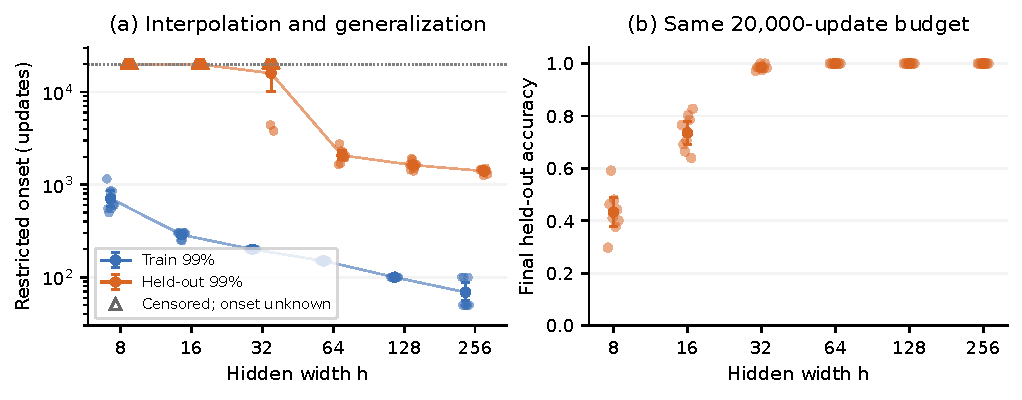
\includegraphics[width=\linewidth]{figures/width.pdf}
\caption{Actual width sweep, eight seeds per width. (a) Sustained 99\% onset, restricted at 19,900 updates; hollow triangles denote non-events, not observed event times. Lines connect restricted means; error bars are seed-bootstrap 95\% CIs. (b) All final held-out accuracies and mean CIs. Every run uses 20,000 updates.}\label{fig:width}
\end{figure}

\begin{table}[t]
\centering\small
\caption{Main sweep. Event counts are out of eight. $\bar T^\tau$ denotes the mean capped endpoint, not an estimated true event time for censored runs. Brackets are unadjusted seed-bootstrap 95\% CIs. Final accuracy uses unprojected logits.}\label{tab:width}
\begin{tabular}{rr r r r r r}\toprule
$h$&Parameters&Train events&$\bar T^\tau_{\rm tr}$&Held-out events&$\bar T^\tau_{\rm ev}$ [CI]&Final (\%)\\\midrule
\inputrows analysis/width_table.tex
\bottomrule\end{tabular}
\end{table}

The width interaction is $\overline D=\WD$ with CI $[\WDLo,\WDHi]$ and adjusted $p=\WPadj$, contradicting W's negative prediction. The separate geometric multipliers on shifted restricted times are \WTrain{} for training and \WGen{} for held-out acquisition; their relative multiplier is \WRelative{} [$\WRelativeLo,\WRelativeHi$]. The latter is emphatically \emph{not} an uncensored generalization-time ratio: six width-32 runs are censored. Recorded training onsets are constant across seeds within each arm (200 versus 100 updates), producing a degenerate bootstrap interval for the shifted-time multiplier; 50-update sampling does not imply zero underlying timing uncertainty.

The result weakens but retains its sign at 95\% ($D=\WNinetyFive$, CI $[\WNinetyFiveLo,\WNinetyFiveHi]$) and 90\% ($D=\WNinety$, CI $[\WNinetyLo,\WNinetyHi]$). These are prespecified secondary sensitivities, not additional corrected discoveries. Width-32 mean final accuracy is \MainSmallEval\%, so missing 99\% often concerns a few errors rather than absence of all rule learning; the primary endpoint is particularly censor-sensitive. Continuous losses and all seed trajectories are retained (Appendix~\ref{app:diagnostics}). Neither the interaction nor the sparse width grid establishes a global monotonic law for raw delay ratios.

An exploratory qualification is important: among the fully observed widths 64 and 256, the same interaction is $D=\WideD$ [\WideDLo,\WideDHi], reversing the primary contrast's sign. Both widths have eight held-out events, so this is not a censored held-out comparison. Across this wider range, fitting accelerates more proportionally even as absolute held-out onset moves earlier. This remains a shifted-time contrast with coarse early fitting samples, not a continuous-rate law. This unadjusted, post-hoc width-range summary does not rescue W's failed frozen 32-to-128 prediction; it demonstrates why that failure is not a global monotonic width law. Appendix~\ref{app:widthgrid} reports every adjacent-grid contrast rather than a selected successful comparison.

\subsection{Clock-compatible first onsets do not imply lasting acquisition}
The shrinkage-clock test separates useful agreement from absence of evidence (Figure~\ref{fig:clock}, Table~\ref{tab:primary}). At width 128 both half- and double-decay arms have eight common-clock events. Their restricted clock difference is $K=\KLarge$ [$\KLargeLo,\KLargeHi$], and the ratio of restricted means is \ClockLargeRestrictedRatio{} [$\ClockLargeRestrictedRatioLo,\ClockLargeRestrictedRatioHi$]. The secondary geometric ratio of fully observed, unshifted clock-event times is \ClockLargeRatio{} [$\ClockLargeRatioLo,\ClockLargeRatioHi$], inside the prespecified 25\% multiplicative margin. This is clock-compatible first-onset evidence, not a universal equivalence theorem or evidence derived merely from a large $p$-value. It does not establish durable acquisition: \HalfLargeRegressions/8 width-128 half-decay runs end below 99\%, with mean final accuracy \HalfLargeFinalMean\% and minimum \HalfLargeFinalMin\%. A post-hoc stability audit (Appendix~\ref{app:stability}) retains the frozen first-event analysis and reports this regression separately; it cannot be hidden by choosing the first successful checkpoint.

At width 32 the half-decay arm has zero common-clock events and the double-decay arm only one. The double-decay arm has four native events over the full update horizon but only one common-clock event: equalizing the clock horizon and persistence changes what is observable. Three common-clock samples span roughly 400 physical updates in the half-decay arm versus 100 in the double-decay arm. These are different estimands, not conflicting counts. Here $K=\KSmall$ [$\KSmallLo,\KSmallHi$] cannot establish collapse: capping forces most pairs to be equal. Neither clock contrast rejects its null after Holm correction. The low-width result remains inconclusive; an inverse clock cannot be assumed there or fitted retrospectively to missing event times. No-decay runs provide finite-budget boundary observations only (Appendix~\ref{app:controls}); they do not establish that explicit decay is universally necessary.

\begin{figure}[t]
\centering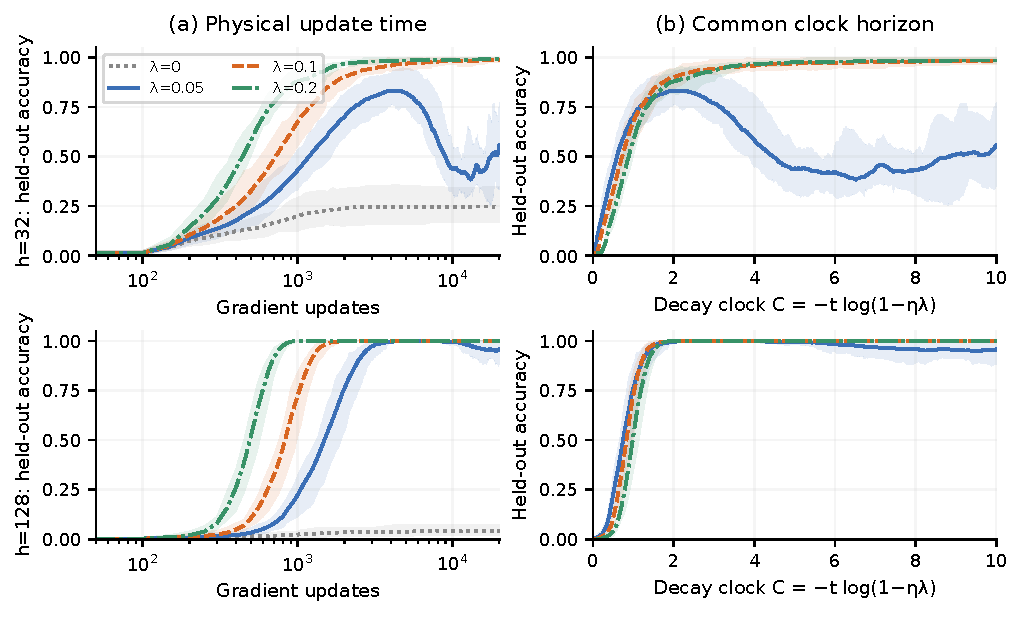
\includegraphics[width=.94\linewidth]{figures/clock.pdf}
\caption{Decay interventions. Curves are mean unprojected held-out accuracy; shaded ranges are seed minima--maxima, \emph{not} confidence intervals. Rows: widths 32 and 128. Left: full update horizon, including zero decay. Right: positive-decay curves on a common clock window, truncated explicitly at $C=10$. Compatible wide-model timing and largely absent narrow-model events are different evidential situations.}\label{fig:clock}
\end{figure}

\begin{table}[t]\centering\small
\caption{All three frozen primary contrasts. W predicts a negative interaction; C predicts a small clock difference. CIs are unadjusted; $p$-values are two-sided. A non-rejection with censored pairs is not equivalence.}\label{tab:primary}
\begin{tabular}{l r r r}\toprule
Contrast&Estimate [95\% CI]&Raw $p$&Holm $p$\\\midrule
\inputrows analysis/primary_table.tex
\bottomrule\end{tabular}\end{table}

\subsection{Parameterization, feature and data controls}
W's observed opposite-direction interaction persists in the secondary raw-mean arm ($D=\NormMeanD$, CI $[\NormMeanDLo,\NormMeanDHi]$) and function-matched mean arm ($D=\NormMatchedD$, CI $[\NormMatchedDLo,\NormMatchedDHi]$). Thus the direction is not removed simply by matching initial logits. Its magnitude and trajectories remain parameterization-dependent; this does not isolate width from optimization. Appendix~\ref{app:controls} reports all control cells, initial-scale comparisons and finite-budget outcomes, including failed transitions, not only successful examples.

Frozen features demonstrate that training fit is insufficient (Figure~\ref{fig:controls}). At width 128 they reach the training threshold in 8/8 runs but have 0/8 held-out events, with final held-out accuracy \FrozenLargeEval\% [\FrozenLargeEvalLo,\FrozenLargeEvalHi]. At width 1024 both trainable and frozen arms fit in 8/8 runs; their final held-out accuracies are respectively \CapacityTrainEval\% and \CapacityFrozenEval\% [\CapacityFrozenEvalLo,\CapacityFrozenEvalHi]. This supports a benefit of feature learning under this recipe without proving universal necessity: freezing also changes optimization and which tensors decay. The width-32 frozen arm underfits and cannot support that inference alone. Shuffled width-128 labels are fitted in 8/8 runs but yield no held-out event; their final shuffled-target accuracy is \ShuffleLargeEval\% [\ShuffleLargeEvalLo,\ShuffleLargeEvalHi].

An explicit width-8 classifier is correct on all 961 pairs at $p=31$ in both float64 and float32, despite random-initialization training never reaching the held-out threshold at that width. This rules out pure lack of representational capacity as a sufficient account of that failure. It does not prove the exact obstruction in the optimizer.

\begin{figure}[t]\centering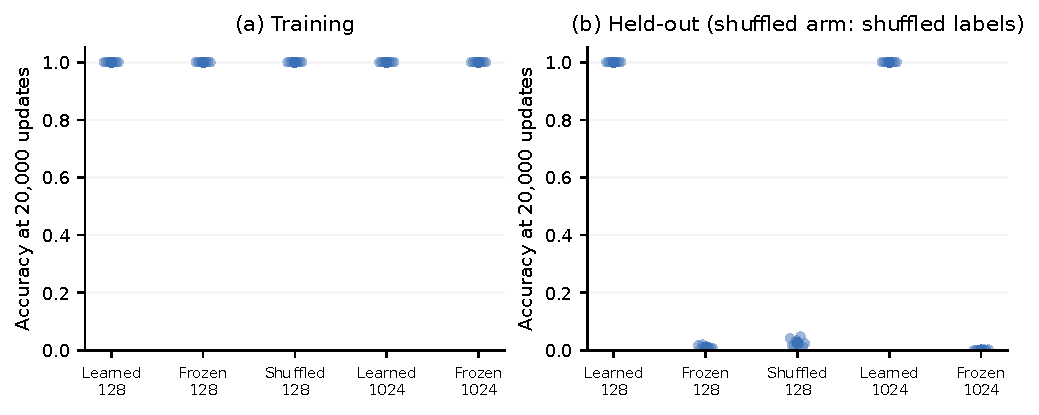
\includegraphics[width=\linewidth]{figures/controls.pdf}
\caption{Trainability and label controls at fixed budget. Dots are individual seeds and bars are bootstrap 95\% CIs. The shuffled arm is evaluated against shuffled labels, not the true modular rule. The width-1024 frozen comparison addresses training capacity directly; the low-width frozen comparison alone cannot identify a feature-learning requirement.}\label{fig:controls}\end{figure}

Lower data fractions give a concrete failure boundary: at $\rho=0.3$, neither width 32 nor 128 has a held-out event despite 8/8 training events each. At $\rho=0.5$, width 128 has 5/8 held-out events versus 0/8 at width 32. At $p=23$, corresponding counts are 8/8 and 1/8. These are secondary findings, not extra confirmatory tests (Appendix~\ref{app:controls}). Changing modulus at fixed fraction changes absolute sample count; subtraction is addition under input relabeling, not an independent algorithm family. The controls therefore cannot support a claim across arbitrary modular operations.

\section{Discussion, Limitations and Conclusion}
The tested memorization-first account is too simple: fitting is already possible at every main width, yet widening from 32 to 128 preferentially accelerates the observable held-out endpoint. The wide model's first-onset clock agreement is conditional and can precede substantial regression. These separate interventions do not establish a causal discovery-then-cleanup pathway or mediation by feature learning. The explicit narrow solution rules out representational impossibility, but does not identify the optimizer's obstruction, prove that no alternative optimizer would work, or establish a sharp width threshold.

There are important limits. Eight paired clusters jointly sample initialization and splitting, not independent variance components. A two-way synthetic split is not an untouched third test set. The 99\% persistence definition, evaluation grid and 20,000-update horizon restrict inference; censored times are unknown, and clock agreement at a wider model does not establish agreement at a narrower one. Normalization and freezing change coordinate dynamics and decay masks, and the oracle projection is neither a trained classifier nor causal mechanism identification. The restricted literature reading prevents unrestricted novelty claims. No transformer, large-model, multiplication or real-data result is supplied.

Within those boundaries the conclusion is falsifiable and empirically supported: width can shorten rather than extend delayed generalization in this recipe, contradicting the primary preferential-interpolation prediction, while the exploratory wide-range comparison reverses the relative interaction. Inverse-decay timing can describe first qualifying onsets without describing lasting generalization. Selecting a model size for a grokking experiment therefore requires checking fit, held-out transitions and subsequent stability, not parameter count or onset time alone.\label{mainend}

\clearpage
\subsection*{AI use statement}
This research artifact was produced unattended by an AI research assistant, including hypothesis formulation, methodology, implementation, CPU execution, statistical analysis, reading the supplied original papers, manuscript drafting, and AI-assisted review. Code and artifacts were checked using unit tests, frozen hashes, event reconstruction and checkpoint evaluation; another AI analysis agent independently audited the width contrast. No human scientific review, human verification of novelty, or exhaustive literature search has occurred, and none is claimed. The artifact is formatted for ICLR 2027 but has not been submitted or accepted. Responsible human authors would need to review all content and satisfy the venue's authorship, disclosure and submission requirements before any actual submission.

\subsection*{Ethics statement}
Data are exhaustive, program-generated arithmetic pairs with no human subjects, personal data or third-party dataset assets. Computation used CPUs only. The main integrity risks are overclaiming from small models, censoring and restricted literature access; the paper and artifact explicitly document these boundaries. No identity or results of the excluded prior work were sought.

\subsection*{Reproducibility statement}
The artifact contains the full training ledger, seeds, dependency versions, generation code, raw trajectories and checkpoints. \texttt{README.md} maps every table and figure to its producing script. \texttt{protocol.json} predates all confirmatory runs; \texttt{experiment\_log.md} records independent pilots, abandoned recipes and access incidents. \texttt{verify\_artifacts.py} recomputes events and verifies hashes, energies, checkpoints and PDF requirements. The exact official template archive and provenance are included for offline compilation.

\bibliography{references}
\bibliographystyle{iclr2027_conference}

\clearpage\appendix
\section{Reproduction, Data Audits and Run Accounting}\label{app:repro}
The host reports Intel Xeon Gold 6230 CPUs at 2.10 GHz and 40 visible logical CPUs; this is not a claim of exclusive allocation. Python 3.11.15, PyTorch 2.15.0+cpu, NumPy 2.4.6 and all remaining package versions are recorded in \texttt{requirements.txt}, with the full installed lock in \texttt{requirements-lock.txt}. Every training process uses one thread. The 240 confirmatory runs consumed \CPUHours{} process CPU-hours during training and diagnostics, excluding interpreter/dependency startup, and the bounded worker launcher took \ElapsedMinutes{} elapsed minutes. Individual measured training-plus-diagnostic wall times ranged from \RunSecondsMin{} to \RunSecondsMax{} seconds under contention. These timings are hardware-dependent, not fixed-compute comparisons.

Exactly 13 exploratory runs are retained separately. Seed 900, width 64, fraction 0.3 and decay 0.1 did not generalize by 12,000 updates. Seed 901 explored widths 32/128, fractions 0.5/0.7 and decays 0.1/1 for 20,000 updates (eight runs). Four validation runs with seeds 902/903, fraction 0.7 and decay 0.1 established early training fit and delayed but partly censored held-out behavior. They motivated the frozen common recipe and are never pooled with seeds 0--7. One additional technical repeat of width 64, seed 0 reproduced all 401 rows and every numerical non-timing column exactly; it is not a new statistical replicate. Thus 254 trained runs are retained in total: 240 frozen, 13 exploratory and one repeat. All exploratory settings and unsuccessful pilot outcomes remain in \texttt{results/pilot}; confirmatory evidence is in \texttt{results/confirm} and the technical repeat in \texttt{results/reproaudit}. No exact transformer reproduction is claimed.

Dataset generation is versioned by the source hash, not an external snapshot. Across all 32 planned $(p,\rho,s)$ split combinations, generation checks find no missing operand value and a minimum training class count of four. Every pair is unique, the subsets are disjoint and exhaustive, and labels follow exact integer arithmetic. The class/operand audit is in \texttt{analysis/data\_audit.json}. Tests cover finite-difference gradients, parameter counts, deterministic splitting, orthogonal projection, function matching, actual AdamW shrinkage and sustained-event/censoring logic. Unit-test arrays are not experimental results.

Source and ledger SHA-256 values are saved in \texttt{protocol.json}; every per-run configuration and summary records the executed source hash, split hash and initial-tensor hash. The final audit requires every planned cell, not merely 240 arbitrary files, and checks all 401 evaluation rows per run. It re-evaluates the actual final checkpoints and verifies all primary and sensitivity event times against the CSVs. Technical errors are distinct from administrative non-events.

\paragraph{Commands and provenance.}
From the workspace root, install \texttt{requirements.txt} and run \texttt{bash reproduce.sh}; with supplied results present, \texttt{bash reproduce.sh --analysis-only} regenerates all analyses, stability and construction checks, figures, numerical TeX inputs and the PDF, then audits them. The complete explicit sequence is in \texttt{README.md}. Existing exact-success command logs allow resumption; to perform fresh training preserve or relocate existing results first as explained there. Training data need no downloads. The selected official ICLR 2027 template permits nine initial main-text pages; bibliography, appendices and the required AI-use statement are excluded. No separate mandatory ICLR checklist is specified in the retrieved guidelines. Venue provenance, unmodified files and a completed artifact-specific reproducibility checklist are included. Formatting is not an actual conference submission.

\section{All Secondary Controls}\label{app:controls}
Figure~\ref{fig:norm} shows the normalization comparison, and Figure~\ref{fig:robust} shows the secondary data/task boundaries. Table~\ref{tab:allcontrols} reports every frozen control cell at the two primary widths, including the reused main baseline, and both width-1024 arms. Train/event counts use sustained 99\%; final accuracy and cross-entropy use the full unprojected classifier and all seed clusters. Brackets around final accuracy are seed-bootstrap intervals, not uncertainty over independent grid entries. No unobserved transition is inserted into a successful-only average.

\begingroup\small\setlength{\tabcolsep}{3pt}
\begin{longtable}{l r r r r r r}
\caption{Complete control ledger outcomes. Main defaults are $p=31,\rho=0.7$, addition, sqrt normalization and decay 0.1; tags denote changes from Table~\ref{tab:ledger}. ``matched'' is function-matched mean; ``modulus'' uses 23; ``lowdata/middata'' use fractions 0.3/0.5. CE is held-out cross-entropy.}\label{tab:allcontrols}\\
\toprule Arm&$h$&$\lambda$&Train events&Held-out events&Final accuracy (\%) [CI]&CE\\\midrule\endfirsthead
\toprule Arm&$h$&$\lambda$&Train events&Held-out events&Final accuracy (\%) [CI]&CE\\\midrule\endhead
\inputrows analysis/controls_table.tex
\bottomrule\end{longtable}\endgroup



\begin{figure}[ht]\centering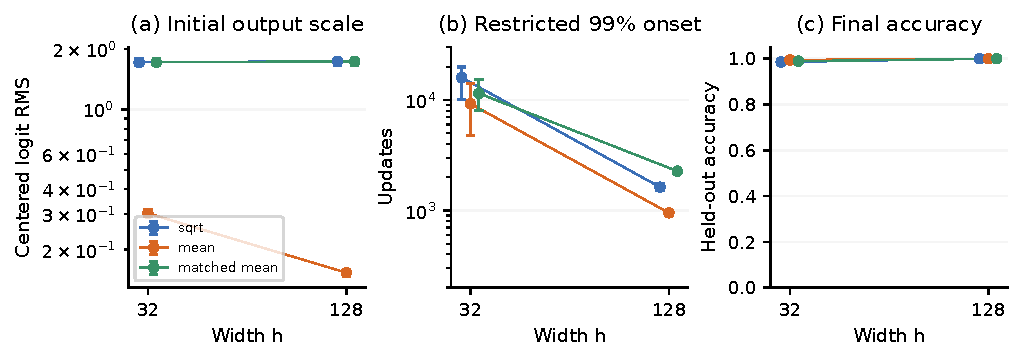
\includegraphics[width=\linewidth]{figures/normalization.pdf}
\caption{Normalization stress tests. ``Matched mean'' reproduces initial sqrt logits, not AdamW coordinate dynamics. Capped event times remain restricted endpoints. Bars are seed-bootstrap 95\% CIs; every arm retains all eight seeds. The similar directional interaction is not invariance of its magnitude or timing.}\label{fig:norm}\end{figure}

\begin{figure}[ht]\centering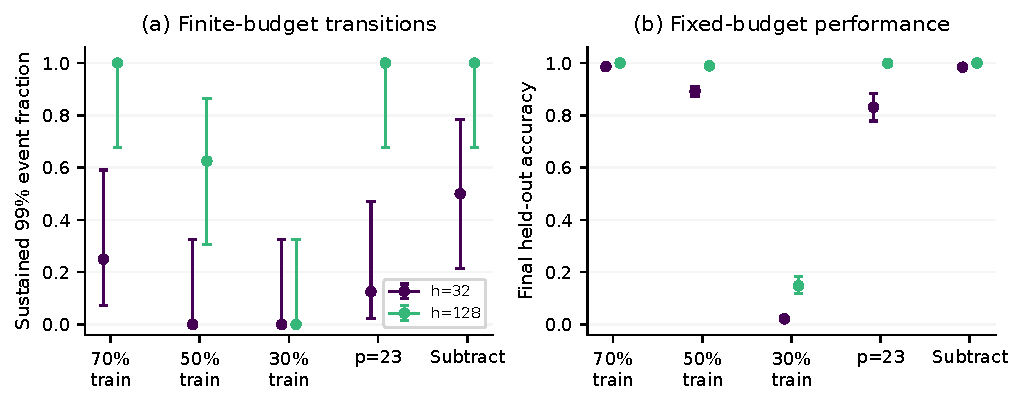
\includegraphics[width=\linewidth]{figures/robustness.pdf}
\caption{Prespecified secondary boundary tests. Event-fraction intervals are Wilson 95\%; final-accuracy intervals are seed-bootstrap 95\%. Changing $p$ changes absolute sample count. Subtraction is an input relabeling of addition. These are not independent confirmations across algorithm families.}\label{fig:robust}\end{figure}

\section{Continuous Trajectories and Rule-Aligned Diagnostics}\label{app:diagnostics}
\begin{figure}[ht]\centering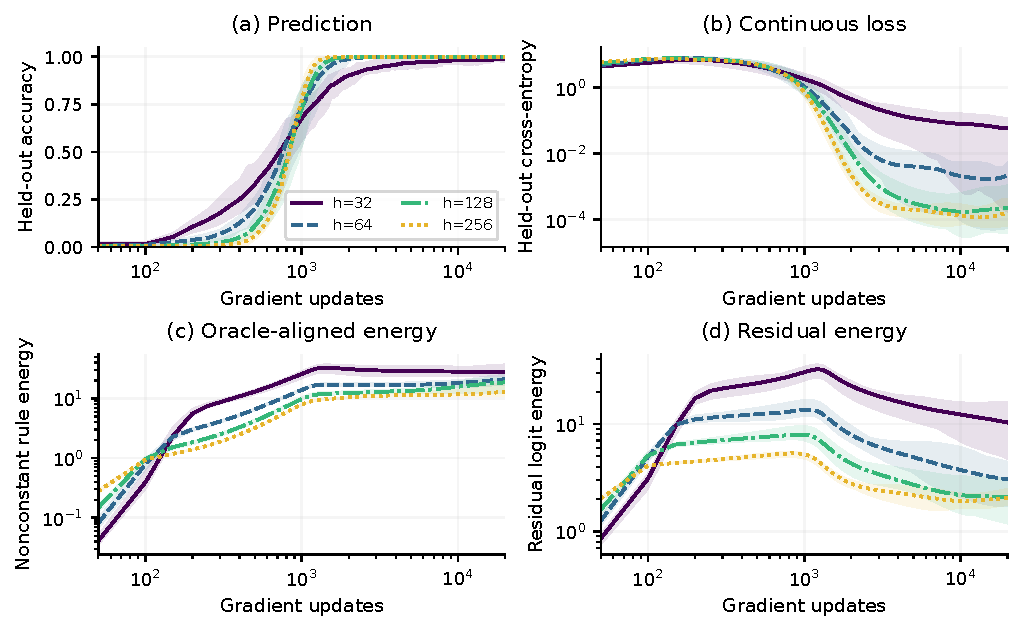
\includegraphics[width=\linewidth]{figures/trajectories.pdf}
\caption{Unprojected prediction and oracle-assisted logit diagnostics. Means and seed minima--maxima over the full horizon (step zero is omitted from logarithmic axes). Rule energy subtracts global class bias; residual energy is the orthogonal complement, not a named memorization circuit. These are post hoc diagnostic plots under a predeclared formula, never training signals or deployable projected accuracies.}\label{fig:diag}\end{figure}

Figure~\ref{fig:diag} reports these diagnostics without identifying a learned circuit. In the uniform full-grid inner product, $\widetilde Z=b+(P\widetilde Z-b)+(\widetilde Z-P\widetilde Z)$ is an orthogonal decomposition. Thus total centered mean-square logits equal the sum of the three absolute logged energies. A growing projected fraction can reflect residual suppression, rule growth or class bias; only logging the fraction would confound them. Projection is over all functions of $r$, not only correct-label or selected-frequency functions. In shuffled runs the grouping rule is still the true arithmetic rule, whereas diagnostic accuracies are against shuffled targets. They cannot be interpreted as recovered rule-classifier performance. No primary conclusion relies on them.

\section{Exact Eight-Unit Construction}\label{app:construction}
Write $x=2\pi a/p$, $y=2\pi b/p$ and $z_c=2\pi c/p$. Four bilinear products give
\begin{align*}
 \cos(x+y-z_c)
 &=\cos z_c(\cos x\cos y-\sin x\sin y)\\
 &\quad+\sin z_c(\sin x\cos y+\cos x\sin y).
\end{align*}
For each product $uv$, two hidden units with operand embeddings $(u,v)$ and $(u,-v)$ give $4uv$ by subtraction. Choose the readout coefficients $\sqrt8/4$ times the respective signed $\cos z_c$ or $\sin z_c$ coefficient. This exactly matches Equation~\ref{eq:model} at $h=8$. The correct residue uniquely maximizes cosine because its angle is zero modulo $2\pi$; every other residue has smaller cosine.

\texttt{verify\_constructive.py} exhaustively checks the resulting non-trained network at primes 23, 31 and 59. It obtains 100\% accuracy on all 529, 961 and 3481 pairs respectively in both float64 and float32. At $p=31$ the measured minimum float64 class margin is 0.02047006 and maximum discrepancy from the direct cosine formula is below $3\times10^{-15}$; these values are saved in \texttt{analysis/constructive.json}. This arithmetic identity and exhaustive check establish existence, not sample-efficient discovery, optimizer accessibility or new learned results. No construction outputs are included among the 240 training runs or their uncertainty estimates.

\section{Post-Hoc Stability Audit}\label{app:stability}
Late regression was noticed while reading completed decay curves. The additional descriptive script \texttt{stability.py} records final-threshold incidence and the first onset whose every remaining recorded accuracy meets 99\%, requiring at least three observations. This persistent-to-end definition is \emph{post hoc}, not a new primary test and not a replacement for frozen events. No additional training or horizon changes were made. Table~\ref{tab:stability} establishes retention only through the observed budget, never permanence beyond it.
\begin{table}[ht]\centering\small
\caption{First qualifying versus persistent-to-end onsets. All counts are out of eight. ``Final99'' means accuracy at the final evaluation reaches 99\%. Mean and minimum final accuracy describe all seeds, not only successful onsets.}\label{tab:stability}
\begin{tabular}{r r r r r r r}\toprule
$h$&$\lambda$&First onsets&Persistent&Final99&Mean final (\%)&Minimum (\%)\\\midrule
\inputrows analysis/stability_table.tex
\bottomrule\end{tabular}\end{table}

\section{Statistical Detail and Interpretation Boundaries}
Every seed-level primary contrast and both sensitivity extractions are preserved in \texttt{analysis/contrasts.json}. The common-clock method uses actual sampled accuracies rather than interpolated predictions. Preceding-evaluation extraction checks timing resolution; the update-5000 landmark keeps all seeds and does not replace the initialization-clock test. Large shared censoring prevents equivalence claims at width 32, regardless of a non-significant sign-flip test. Where all events are observed at width 128, the reported clock-ratio compatibility interval is a secondary, unadjusted interval within a stated margin, not a separately powered confirmatory equivalence test.

\subsection{Exploratory width-grid contrasts}\label{app:widthgrid}
The remaining-width contrasts were designated secondary in the freeze. After examining the complete grid, we summarize all adjacent pairs and the 64-to-256 range, where every seed reaches the held-out event. These comparisons are exploratory and their intervals unadjusted; there is no additional confirmatory family or change to W's prespecified 32-to-128 test. Capping and the +50 offset have exactly the meanings in Equation~\ref{eq:width}.
\begin{table}[ht]\centering\small
\caption{Exploratory width contrasts under the same shifted, capped endpoint. Negative $D$ means greater relative acceleration of training; positive $D$ means greater relative acceleration of held-out onset. The fully observed wide-range reversal does not establish a universal transition width.}\label{tab:widthgrid}
\begin{tabular}{l r}\toprule Width change&$D$ [unadjusted 95\% CI]\\\midrule
\inputrows analysis/secondary_width_table.tex
\bottomrule\end{tabular}\end{table}
Table~\ref{tab:widthgrid} exposes sign and magnitude changes across the grid. For 8-to-16 both held-out arms are entirely censored, so negative $D$ reflects faster fitting against a shared cap, not an observed grokking delay. The 64-to-256 comparison has no held-out censoring. These are descriptive boundaries for the author-formulated account, not causal evidence of a new serial mechanism.

Percentile bootstrap intervals resample eight seed clusters, never individual pairs or evaluations. At this small sample size they are approximate and can be discrete; sign-flip tests additionally assume symmetry/exchangeability under the null. The minimum possible two-sided sign-flip $p$ with eight nonzero equally signed pairs is $2/256$, so the primary width evidence is at the resolution limit of that test. The underlying 50-update accuracy grid likewise limits time precision. True event times beyond administrative censoring are not recovered by the restricted endpoint, and no population scaling exponent is fitted.

\section{Independent Literature Access Boundary}
Only the seven cited, user-supplied original arXiv PDFs were consulted, using direct URLs. No topical, citation or repository search was performed. References within the allowed originals were not followed. Official template and policy pages were retrieved separately, without entering paper listings. No known accidental forbidden exposure was detected; because the excluded work was undisclosed, this is a statement of access procedures, not an identification-based guarantee. \texttt{literature/ACCESS\_AUDIT.md}, \texttt{literature\_notes.md} and \texttt{template/PROVENANCE.md} record URLs, versions, pages actually read, hashes and failed direct template URL probes. This boundary deliberately limits novelty assessment and does not weaken the need to acknowledge prior model-wise grokking in the permitted sources.
\end{document}
